\section{Grundlagen}
%- Wissenschaftlicher Stand
\subsection{Architektur AR Anwendungen}
\subsection{Haptische Interaktionsmethoden in VR Umgebungen}
\subsection{Handtracking Interaktionsmethoden}
\subsection{Menüführung in VR Umgebungen}
\subsection{Datenaustausch über internes Netzwerk}

\subsection{Green-Keying}\label{sec:Green-Keying}
\subsection{Marker Tracking} \label{sec:MarkerTracking}\todo[inline]{Vera}
In einer VR Umgebung werden zur interaktiven Steuerung der Position und Orientierung eines 3D Objektes sogenannte Marker benötigt. Mit Hilfe dessen können die aktuellen Positionen in der Realität in einem Kamerabild erfasst werden und in den erforderlichen 3D-Raum transformiert werden. Diese Marker bestehen aus eindeutigen Codes, welche in der Regel in Form von binären Muster verwendet werden. In Abbildung \ref{fig:BinMarker} sind vielfältige Beispiele von binären Codes zu sehen, die zum Marker Tracking verwendet werden. Jedem Code wird eine unverwechselbaren ID zu geordnet um Überschneidungen zu vermeiden und jeden Marker auch nach längerer Verdeckung eindeutig identifizieren und orten zu können.\\
Zur eindeutigen Identifizierung von den Codes sind vielfältige Schritte notwendig. Zunächst muss das Muster innerhalb eines Bildes oder Videos erkannt, geortet und verifiziert werden. Im Anschluss wird das gültige Muster der entsprechenden Identifikation (ID) zu geordnet sowie die Orientierung des Markers im Kameraraum berechnet. Diese umfangreichen Ermittlungsprozesse werden in der Regel von entsprechenden Bibliotheken zur Verfügung gestellt, wie zum Beispiel das \textit{ArUco} Modul (siehe Kapitel \ref{sec:aruco}) aus dem Bildverarbeitungsbibliothek \textit{OpenCV} (siehe Kapitel \ref{sec:OpenCV}). \\
\begin{figure}[H] 
	\center 
	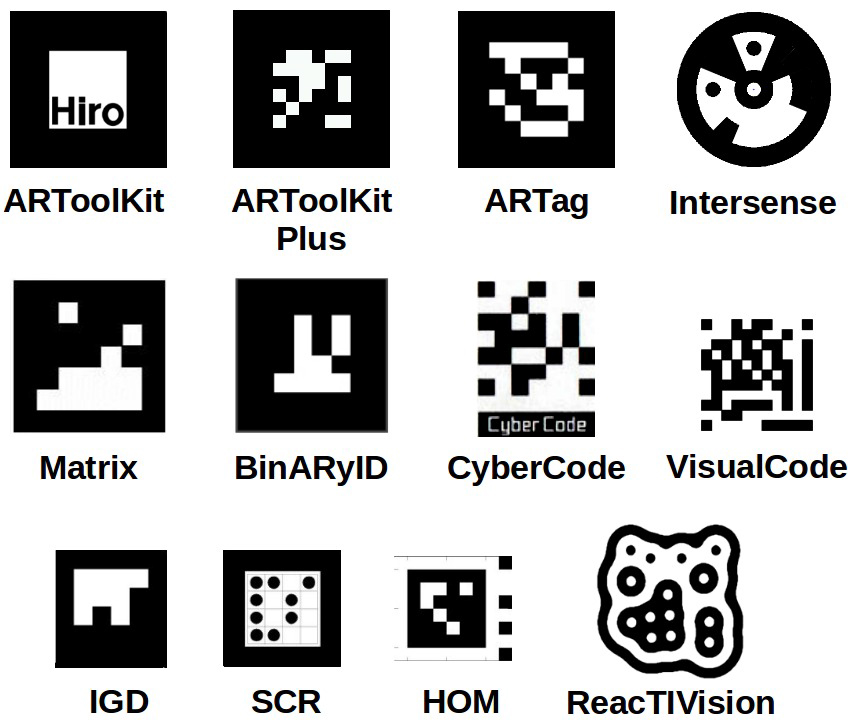
\includegraphics[width=8cm]{Bilder/BinMuster.jpg}			
	\caption{Diverse Binäre Muster die als Code für Marker Tracking verwendet werden. Quelle: \cite{article:Aruco2014}}
	\label{fig:BinMarker}
\end{figure}
